\chapter{Správa dat v architektuře mikroslužeb}\label{ch:msa-data}

\chaptersummary{
   \begin{ul}
      \item způsoby integrace datových zdrojů do \g{MSA},
      \item spojování dat napříč mikroslužbami,
      \item transakční zpracování napříč mikroslužbami.
   \end{ul}
}

Databáze jako datový zdroj je jednim z možných řešení pro persistentní ukládání dat s případným následným zpracováním.
Daná kapitola je věnována především dvěma návrhovým vzorům pro organizaci dat v relačních databázích dodržujících \g{ACID} vlastnosti a spolupráci mikroslužeb pro vyhodnocování pokročilých klientských požadavků.
Popisované databázové organizace dat se obecně nemusí týkat pouze architektury mikroslužeb, ale nachází zde svoje přímé uplatnění.



\section{Typy organizace zdrojů}\label{sec:msa-db-as-data-source}

V jednoduché monolitní architektuře využití relační databáze může být zcela přímočaré – jeden monolit se připojuje k jedné databázi, která spravuje veškerá potřebná data.
Mikroslužby však představují separaci na jednotlivé částí dle zvolené dekompozice a intuitivně přináší i myšlenku dělení původně jednoho datového zdroje na obdobně dekomponované celky.
Ná základě této uvahy můžeme definovat dva návrhové vzory pro organizaci dat:

\begin{dl}
   \item [Sdílená databáze (ShDB)] – jedna instance databáze je plně přístupna pro všechny připojemé mikroslužby~\cite{shareddb}.
   \item [Databáze pro každou službu (DBpS)] – každá deklarovaná mikroslužba používá vlastní databázi (nebo schémata), do které má výhradní přistup~\cite{dbperservice}.
   V takovém případě se samozřejmě může jednat i o fyzicky samostatné databázové servery.
\end{dl}

Oba přístupy mají svoje využití dle poskytovaných vlastností.



\subsection{Sdílená databáze}\label{subsec:shared-db}

Sdílená databáze poskytuje všechna svoje úložiště všem mikroslužbám, možná realizace je znázorněna na obrázku~\ref{fig:db-shared}. \g{ACID} vlastnosti zde jsou řízeny databází a logicky se ničím neliší od komunikací s monolitickou aplikací.

\begin{figure}[htbp]
   \centering
   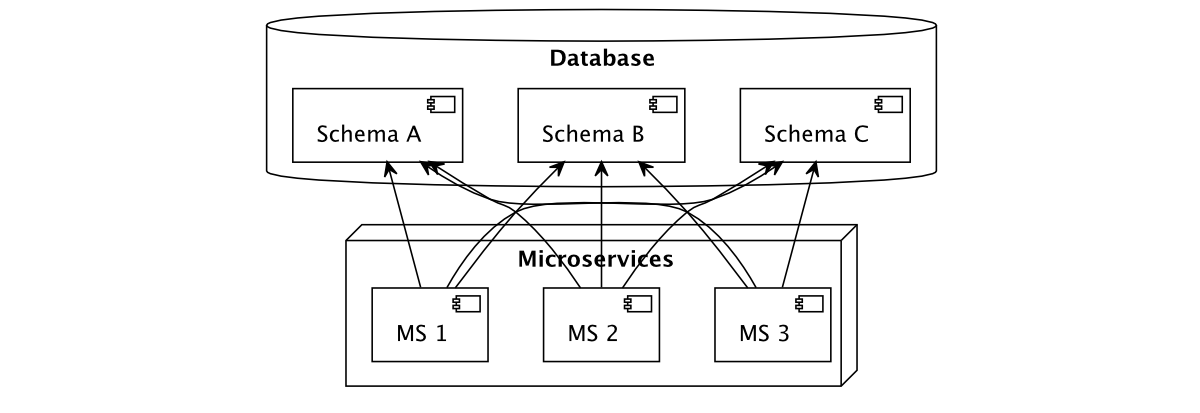
\includegraphics[max width=\textwidth]{assets/db-shared}
   \caption{Architektura sdílené databáze}\label{fig:db-shared}
\end{figure}

Výhody
\begin{ul}
   \item Typické použití \g{ACID} pro provádění transakcí~\cite{shareddb}.
   \item Správa jedné databáze je jednodušší~\cite{shareddb}.
\end{ul}

Nevýhody
\begin{ul}
   \item Databázové migrace se netýkají pouze jedné mikroslužby, ale všech zároveň, musí se vyčlenit místo pro jejich uchovávání.
   \item V případě jakékoliv změny struktury databáze je třeba změnit a otestovat všechny mikroslužby~\cite{shareddb}.
   \item Jednotná databáze nemusí vyhovovat potřebám všech mikroslužeb~\cite{shareddb}.
\end{ul}



\subsection{Databáze pro každou službu}\label{subsec:msa-db-per-service}

V případě vyčlenění jednoho schématu, či celé databáze pro každou mikroslužbu, můžeme mluvit o druhým typu struktury využití relačních databází, možná realizace je zázorněna na obrázku~\ref{fig:db-per-micro}.

\begin{figure}[htbp]
   \centering
   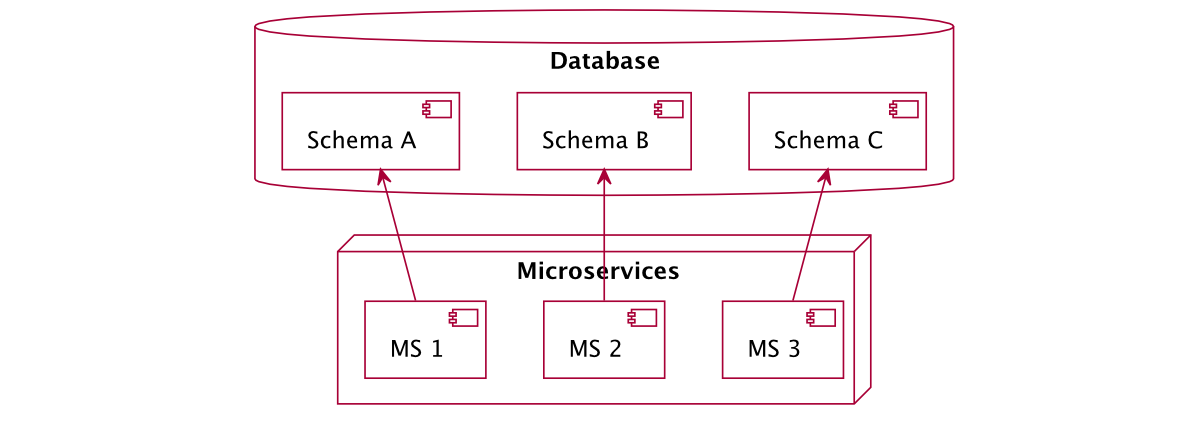
\includegraphics[max width=\textwidth]{assets/db-per-micro}
   \caption{Architektura databází (schémat) pro každou službu}\label{fig:db-per-micro}
\end{figure}



Výhody
\begin{ul}
   \item Zmenšení provázanosti mikroslužeb a dat, jež jsou využívány – lepší správa migrací a jiných změn~\cite{dbperservice}.
   \item Lepší možnosti škálování a volby databáze – mikroslužbě je možné poskytnout takové prostředí, které bude nejvhodnější~\cite{dbperservice}.
\end{ul}

Nevýhody
\begin{ul}
   \item Problém se spojováním dat z více úložiští – nelze například provádět \h{JOIN}, párovat dle cizího klíče s kontrolou integritního omezení~\cite{dbperservice}.
   \item Problém s transakčním zpracováním – transakční operace nad několika databázemi nelze jednoduše provádět a je lepší se jim úplně vyhýbat~\cite{dbperservice}.
   \item Komplikovaná správa a konfigurace většího počtu databází~\cite{dbperservice}.
\end{ul}

Nevýhody databází rozdělených dle mikroslužeb lze řešit s pomocí některých návrhových vzorů, jsou ve stručnosti popsány v následujích podkapitolách.



\section{Spojování dat mezi mikroslužbami}\label{sec:msa-db-join}
Jako jeden z možných požadavků v rámci \g{MSA} je spojení dat mezi tabulkami, což v rámci oddělených služeb znamená netriviální úkol.
Jako typický příklad lze vzít existenci tabulek \h{users} (osobní informace) a \h{payments} (částky a primárního klíče z \h{users}), jež se nachází v oddělených databázích, ze kterých je třeba získat seznam transakcí všech lidí s určitým věkem.
Spojení v tomto případě nemůžeme nechávat na databázi, situace se může řešit API kompozicí nebo \g{CQRS}.



\subsection{API kompozice}\label{subsec:msa-db-aggregate-api}



\subsection{CQRS}\label{subsec:msa-db-aggregate-cqrs}



\section{Transakční zpracování zápisů}\label{sec:msa-db-transaction}

U databází na principu \g{ACID} může při některých pořadavcích docházet k porušení izolace a je třeba zajistit konzistenci.
Informace o ságách a využití.
Sagy, neboli příběhy, zajištují transakční zpracování napříč databázemi.



\subsection{Koordinace ságy choreografie}\label{subsec:msa-db-transaction-coordinate-choreography}



\subsection{Koordinace ságy orchestrace}\label{subsec:msa-db-transaction-coordinate-orchestration}
